\documentclass{beamer}
\usepackage[T2A]{fontenc}
\usepackage[utf8]{inputenc}
\usepackage{amssymb,amsfonts,amsmath,mathtext,cite,enumerate,float,gensymb}
\usepackage{colortbl}
\usetheme{Warsaw}
\title[SIFT та ASIFT для співставлення зображень]{Використання алгоритмів SIFT та ASIFT для співставлення зображень}
\author{Євген Варавва -- ННК ``ІПСА'' НТУУ ``КПІ''}
\institute{XII Міжнародна науково-технічна конференція САІТ-2010}
\date{26 травня, 2010}
\usepackage{graphicx}
\graphicspath{{images/}}
\begin{document}

\newcommand{\coolfigure}[3]{\coolwfigure{#1}{#2}{#3}{\textwidth}}

\newcommand{\coolwfigure}[4]{\begin{figure}[!ht]\begin{center}\includegraphics[width=#4]{#1}\end{center}\caption{#2}\label{#3}\end{figure}}


\AtBeginSubsection[]
{
  \begin{frame}<beamer>
  \frametitle{Layout}
  \tableofcontents[currentsection,currentsubsection]
  \end{frame}
}

\begin{frame}
  \titlepage
\end{frame}


\begin{frame}{Автоматична обробка зображень (Комп'ютерний зір)}
  \begin{itemize}
    \item Системи спостереження
    \item Потокового телебачення
    \item Медичні дослідження
      \begin{itemize}
        \item мікроскопічні
        \item рентгенівські
        \item ангіографічні
        \item ультразвукові
      \end{itemize}
    \item Військова галузь
      \begin{itemize}
        \item Автоматичне керування 
        \item Навігація на основі моделей, побудованих в реальному часі
      \end{itemize}
  \end{itemize}
\end{frame}

\begin{frame}{Типові задачі комп'ютерного зору}
  \begin{itemize}
    \item Розпізнавання
      \begin{itemize}
        \item Розпізнавання об'єктів
        \item Ідентифікація
        \item Виявлення
      \end{itemize}
    \item Аналіз руху
      \begin{itemize}
        \item Постійний рух
        \item Трекінг
        \item Оптичний плин
      \end{itemize}
    \item Відновлення 3D сцен
    \item Відновлення зображень
  \end{itemize}
\end{frame}

\begin{frame}{Постановка задачі}
  За заданими еталонними зображеннями об'єкта вказати, дослідити присутність об'єкта на досліджуваному зображенні
\end{frame}

\begin{frame}{Загальий огляд досягнень}
  Пошук локальних особливостей -- важливі події
  \begin{itemize}
    \item Моравіц (1981) -- з ``детектором кутів'' Гарріса % вибирають частини, що мають великі градієнти у всіх напрямах
    \item Шмід та Мор (1997) -- співставлення с великою базою еталонних зображень зі змінними кутами, зашумленістю, маючи лише частину зображення
    \item Лов (1999) -- інваріантність відносно масштабу
  \end{itemize}
  \pause Інші типи особливостей зображень
  \begin{itemize}
    \item контури, границі об'єктів
    \item багатовимірні гістограми, що описують виміри по частинах зображення
    \item колір, рух, опис регіонів зображення
  \end{itemize}
\end{frame}

\begin{frame}{Алгоритм SIFT}
  Описує особливості зображення інваріантно, відносно:
  
\includegraphics{transf-orig} \\
  \begin{tabular}{ccc}
    позиції & повороту & масштабування \\
    
\includegraphics{transf-pos} & \includegraphics{transf-rotate} & \includegraphics{transf-scale} \\
  \end{tabular}

  Забезпечує стійкість до
  \begin{tabular}{ccc}
    афінних спотворень & змін 3D точки зору & змін рівню шуму, освітленості \\
    \includegraphics{transf-affine} & \includegraphics{transf-cammove} & \includegraphics{transf-noise} \\
  \end{tabular}
\end{frame}

\begin{frame}{Власне алгоритм}
  \begin{enumerate}
    \item Визначення екстремумів в масштабно-просторовому представленні
    \item Локалізація ключових точок
    \item Визначення орієнтації
    \item Побудова дескрипторів ключових точок
  \end{enumerate}
\end{frame}

\begin{frame}{Екстремуми в масштабно-просторовому представленні зображення}
  У якості МПП -- згортка гаусівської функції з вихідним зображенням:
  \[
  L(x,y,\sigma) = G(x,y,\sigma) \ast I(x,y)
  \]

  де $\ast$ -- оператор згортки по $x$ та $y$, а

  \[
    G(x,y,\sigma) = \frac{1}{2\pi\sigma^2}e^{-(x^2+y^2)/2\sigma^2}.
  \]
\end{frame}

\begin{frame}{Уточнення позицій ключових точок}
  Розклавши в ряд Тейлора:
  \begin{equation}
    \label{eq:d-taylor}
    D(\mathbf{x}) = D + {\frac{\partial D}{\partial \mathbf{x}}}^T \mathbf{x} + \frac12 \mathbf{x}^T \frac{\partial ^2 D}{\partial\mathbf{x}^2}\mathbf{x}
  \end{equation}

  Звідки можна оцінити $\hat{\mathbf{x}}$:

  \begin{equation}
    \label{eq:extr-ext}
    \hat{\mathbf{x}} = -\left(\frac{\partial^2 D}{\partial \mathbf{x}^2}\right)^{-1} \frac{\partial D}{\partial \mathbf{x}}
  \end{equation}

  де $D$ та всі відповідні похідні визначаються в досліджуваній точці вибірки, а $\mathbf{x} = (x,y,\sigma)^T$.
\end{frame}

\begin{frame}{Відшукання орієнтації ключових точок}
  \begin{itemize}
    \item $L$ -- розмите зображення
    \item $m(x,y)$ -- довжина градієнту
    \item $\theta(x,y)$ -- орієнтація
  \end{itemize}

  \[
    m(x,y) = \sqrt{(L(x+1, y) - L(x-1, y))^2 + (L(x,y+1) - L(x,y-1))^2} 
  \]

  \[
    \theta(x,y) = \tan^{-1}((L(x,y+1) - L(x,y-1)) / (L(x+1,y) - L(x-1,y)))
  \]

  Піки гістограми орієнтацій градієнтів точок, що оточують досліджувану -- орієнтації ключової точки
\end{frame}

\begin{frame}{Побудова SIFT-дескрипторів}
  \begin{figure}[h]
    \begin{minipage}[h]{0.49\linewidth}
      \center{\includegraphics[width=0.5\linewidth]{sift-local-gradients} \\
      Довжини і напрямки локальних градієнтів у кожній точці в квадратній області навколо досліджуваної. Вони зважуються гаусівським вікном, що позначене синім колом.
      }
    \end{minipage}
    \hfill
    \begin{minipage}[h]{0.49\linewidth}
      \center{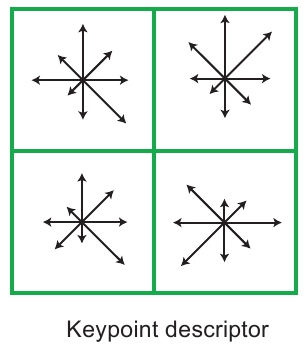
\includegraphics[width=0.5\linewidth]{sift-keypoint-descriptor} \\
      Значення локальних градієнтів з областей $4\times4$ збираються в гістограми з 8-и елементів. Довжини стрілок відповідають сумі довжин локальних градієнтів, близьких за напрямом, в рамках відповідної області.
      }
    \end{minipage}
    \label{fig:sift-descriptor}
  \end{figure}
\end{frame}

\begin{frame}{Приклад роботи алгоритму SIFT}
  \begin{figure}[h]
    \begin{minipage}[h]{0.49\linewidth}
      \center{
      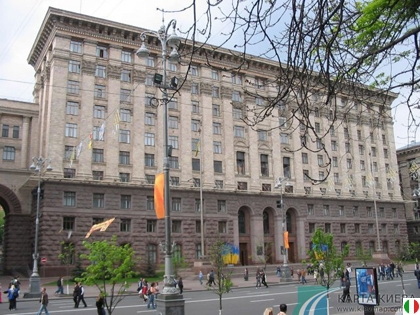
\includegraphics[width=\linewidth]{meria-vhod} \\
      \includegraphics[width=\linewidth]{meria-arka} \\
      }
    \end{minipage}
    \hfill
    \begin{minipage}[h]{0.49\linewidth}
      \center{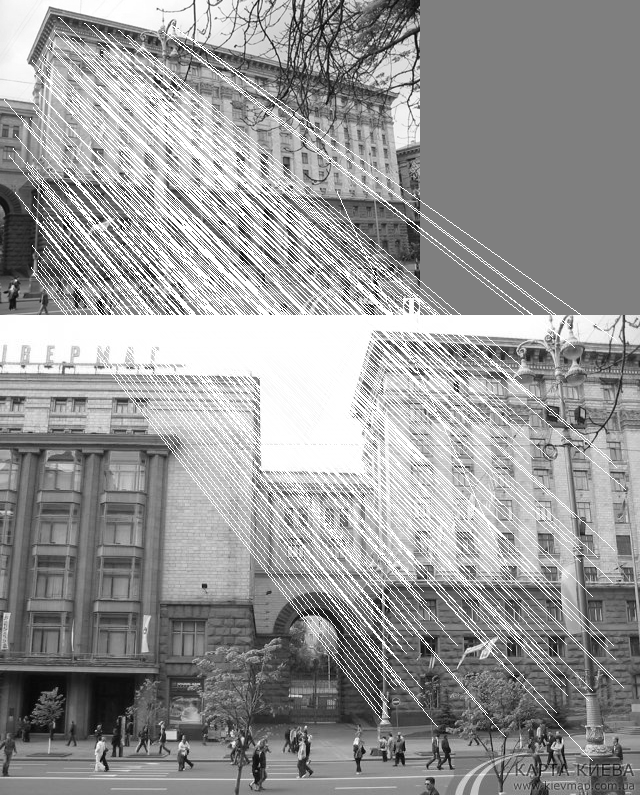
\includegraphics[width=\linewidth]{sift-out} \\
      }
    \end{minipage}
    %\caption{Побудова SIFT-дескрипторів}
    \label{fig:sift-sample}
    \caption{Приклад порівняння зображень за допомогою SIFT.}
  \end{figure}
\end{frame}

\begin{frame}{ASIFT}
  Розглядає наступну модель отримання зображення:

  \begin{center}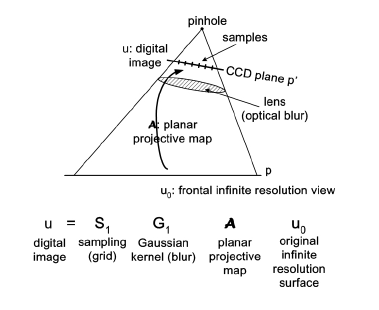
\includegraphics[width=0.3\linewidth]{camera-model}\end{center}

  \begin{equation}
    \textbf{u}=\textbf{S}_1G_1A\mathcal{T}u_0
  \end{equation}

  \begin{itemize}
    \item $\textbf{u}$ -- отримане цифрове зображення
    \item $u_0$ -- нескінченний фронтальний вигляд плоского об'єкта
    \item $\mathcal{T}$ та $A$ -- відповідно зміщення та плоска проекція, пов'язані з переміщенням камери
    \item $G_1$ -- гаусівська згортка, що моделює оптичне розмиття
    \item $\textbf{S}_1$ -- оператор дискретизації зображення на сітці з кроком 1
  \end{itemize}
\end{frame}

\begin{frame}
  Апроксимуємо оператор $A$ афінним перетворенням. Тоді, має місце розклад:
  \begin{equation}
    \label{eq:asift-decomposition}
    A = H_\lambda R_1(\psi)T_tR_2(\phi) =     
    \lambda \begin{bmatrix} 
      \cos \psi & -\sin\psi \\
      \sin\psi  & \cos\psi
    \end{bmatrix}
    \begin{bmatrix}
      t & 0 \\
      0 & 1 
    \end{bmatrix}
    \begin{bmatrix} 
      \cos \phi & -\sin\phi \\
      \sin\phi  & \cos\phi
    \end{bmatrix}
  \end{equation}

  де $\lambda>0$, $\lambda t$ -- визначник матриці $A$, $R_i$ -- повороти, $\phi \in \left[0,\pi\right)$, та $T_t$ -- нахил, що є діагональною матрицею з власними числами $t>1$ та 1.

  геометрична інтерпретація розкладу:
  \begin{center}\includegraphics[width=0.2\linewidth]{asift-decomposition}\end{center}
  \begin{itemize}
    \item $\phi$ та $\theta= \arccos1/t$ -- кути огляду
    \item $\psi$ параметризує обертання камери
    \item $\lambda$ відповідає масштабу
  \end{itemize}

\end{frame}

\begin{frame}{Власне алгоритм ASIFT}
  \begin{itemize}
    \item Симуляція спортворень, викликаних відхиленням осі камери від фронтального положення
    \begin{center}\includegraphics[width=0.8\linewidth]{asift-sampling}\end{center}
    \item Отримані в результаті симуляції зображення порівнюють за допомогою деякого алгоритму (SIFT)
  \end{itemize}
\end{frame}

\begin{frame}{Оптимізація ASIFT}
  \begin{itemize}
    \item Зменшення досліджуваного та еталонного зображення в K$\times$K разів
    \item Застосування алгоритму ASIFT, описаного вище, до зменшених зображень
    \item Вибір $M$ афінних перетворень, що дають найбільшу кількість збігів на зменшених зображеннях
    \item Застосування ASIFT до повнорозмірних зображень, але симулювати лише $M$ афінних перетворень.
  \end{itemize}
\end{frame}

\begin{frame}{Порівняння ASIFT та SIFT}
  \coolwfigure{asift-graffiti}{Два зображення графіті з відносним нахилом $\tau \approx 3.2$. ASIFT та SIFT знайшли, відповідно, 925 і 2 правильних співпадіння.}{fig:asift-graffiti}{0.5\linewidth}
\end{frame}

\begin{frame}{Порівняння ASIFT та SIFT}
  \coolwfigure{asift-scale}{Реакція алгоритмів на зміни масштабу: ASIFT, SIFT -- 221 та 86 вірних співпадінь відповідно.}{fig:asift-scale}{0.6\linewidth}
\end{frame}

\begin{frame}{Порівняння ASIFT та SIFT}
    \begin{center}\includegraphics[width=0.7\linewidth]{asift-near}\end{center}
  Відповідність між двома зображеннями картини, отриманими з фронтального виду та під кутом $75\degree$. ASIFT -- 202, SIFT -- 15 вірних точок.
\end{frame}

\begin{frame}{Порівняння ASIFT та SIFT}
  \coolwfigure{asift-magazine}{Відповідність між двома зображеннями журналу, з масштабом $\times 4$, отриманими з фронтального виду та під кутом $80\degree$. ASIFT -- 349, SIFT -- 0 вірних точок.}{fig:asift-magazine}{0.5\linewidth}
\end{frame}

\begin{frame}{Порівняння ASIFT та SIFT}
  \coolwfigure{asift-longitude}{Відповідність між двома зображеннями журналу, що відрізняються кутом довготи на $50\degree$. ASIFT -- 745, SIFT -- 3 вірних точок.}{fig:asift-longitude}{0.5\linewidth}
\end{frame}


\begin{frame}{Порівняння ASIFT та SIFT}
  \coolwfigure{asift-road}{Відповідність між двома зображеннями дорожного знаку. Відносний нахил $\tau \approx 2.6$. ASIFT -- 50, SIFT -- 0 вірних точок.}{fig:asift-road}{0.5\linewidth}
\end{frame}


\end{document}
